\chapter{Interfaces de Usuario}
\label{app-interfacesdeusuario}

En este ap�ndice se presentar�n las principales interfaces con la que el usuario trabajar�. Todo esto con el fin de visualizar los elementos gr�ficos que ayudar�n al usuario a manejar y solicitar las funciones del sistema. A continuaci�n se muestran algunas interfaces de usuario. Para ver m�s interfaces, ir a la Secci�n \ref{casosdeusosreales} sobre Casos de Usos Reales. \\

\begin{itemize}

\item \textbf{Interfaz Ventana Inicial:} Interfaz com�n que ver�n todos los usuarios que ingresen al sistema. �sta permite al usuario crear una cuenta de alumno o ingresar directamente al Sistema. Ver Figura \ref{fig:login}. \\

\item \textbf{Interfaz Inicial de Usuario Profesor:} Muestra la interfaz de inicio del Profesor. Contiene el men� con acceso a las funciones principales que �ste posee. Ver Figura \ref{fig:usuarioprofesor}. \\

\item \textbf{Interfaz Inicial de Usuario Alumno:} Muestra la interfaz de inicio del Alumno. Contiene el men� con acceso a las funciones principales que �ste posee. Ver Figura \ref{fig:usuarioalumno}. \\

\item \textbf{Interfaz Crear Cuenta Alumno:} Interfaz que contiene la interfaz para le creaci�n de una cuenta como alumno desde la sesi�n del Profesor. Ver Figura \ref{fig:crearcuentaprofesor}. \\

\item \textbf{Interfaz Cargar BD:} Interfaz que muestra una lista de bases de datos disponibles para ser cargadas al sistema. Cualquier usuario registrado puede acceder a esta interfaz. Ver Figura \ref{fig:cargarbd}. \\

\item \textbf{Interfaz Hacer Consulta:} Muestra la interfaz para hacer consultas en �lgebra Relacional a una base de datos cargada. Cualquier usuario registrado puede acceder a esta interfaz. Ver Figura \ref{fig:hacerconsulta}. \\

\item \textbf{Interfaz Crear Ejercicios:} Muestra la interfaz para la creaci�n de ejercicios para una base de datos cargada. Solo el usuario Profesor puede acceder a esta interfaz.  Ver Figura \ref{fig:crearejercicios}. \\

\item \textbf{Interfaz Responder Ejercicios:} Interfaz que contiene el formulario para el desarrollo de ejercicios dise�ados para cada base de datos. Cualquier usuario registrado puede acceder a esta funcionalidad. Ver Figura \ref{fig:responderejercicios}. \\

\end{itemize}

\clearpage
\begin{figure}[h!]
\centering
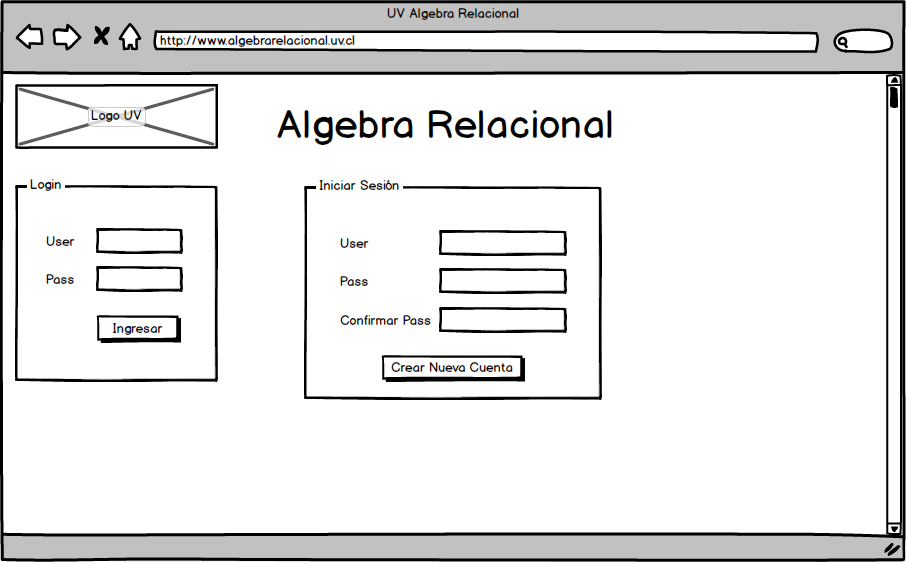
\includegraphics[width=13cm]{imagenes/login.png}
\caption{Interfaz Ventana Inicial.}
\label{fig:login}
\end{figure}

\begin{figure}[h!]
\centering
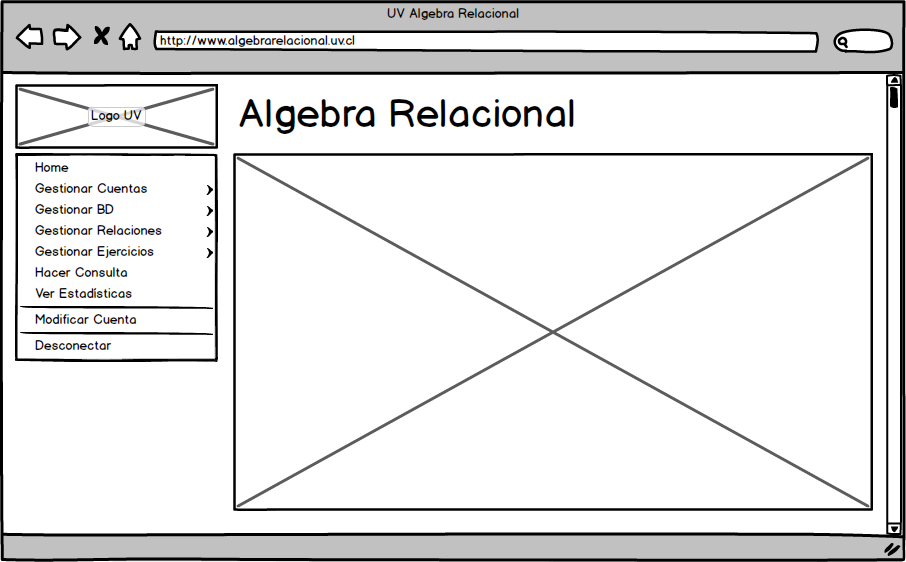
\includegraphics[width=13cm]{imagenes/usuario_profesor.png}
\caption{Interfaz Inicial de Usuario Profesor.}
\label{fig:usuarioprofesor}
\end{figure}

\clearpage
\begin{figure}[h!]
\centering
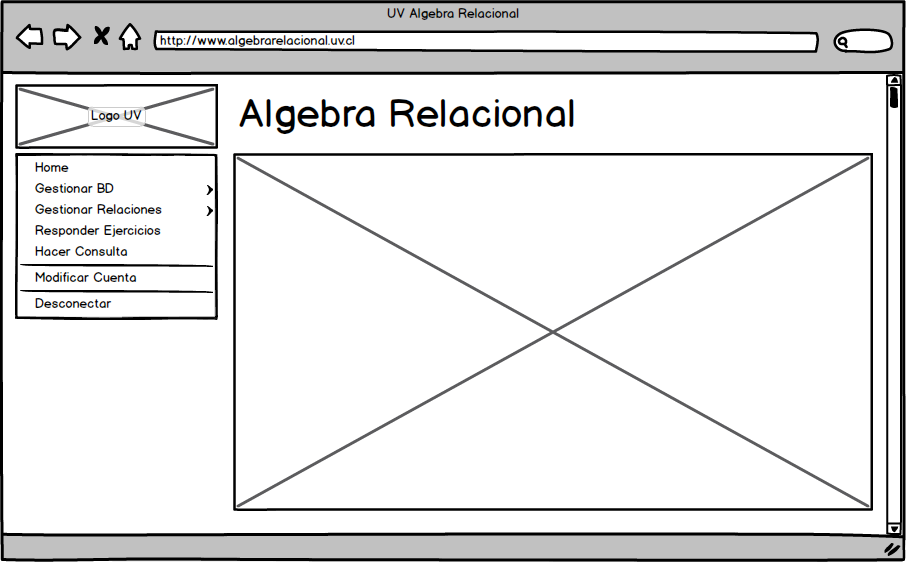
\includegraphics[width=13cm]{imagenes/usuario_alumno.png}
\caption{Interfaz Inicial de Usuario Alumno.}
\label{fig:usuarioalumno}
\end{figure}

\begin{figure}[h!]
\centering
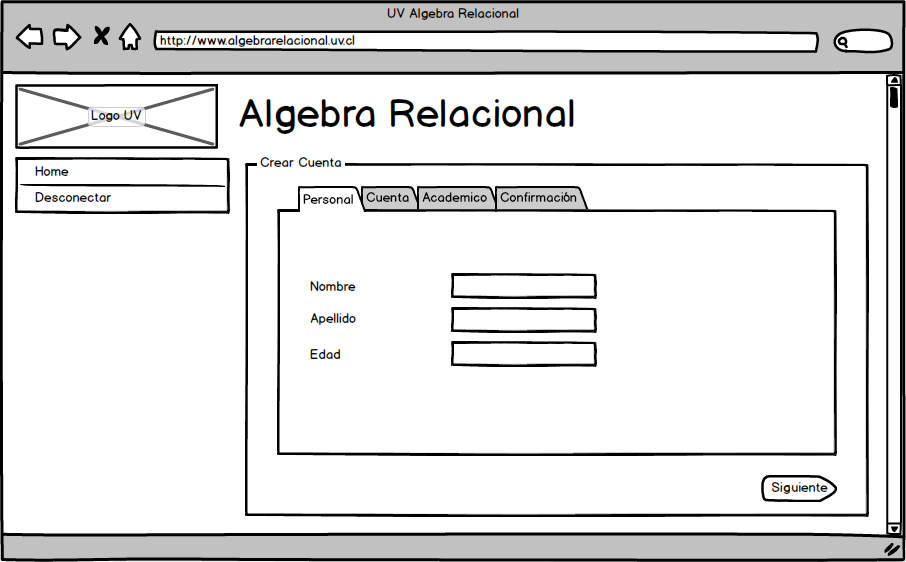
\includegraphics[width=13cm]{imagenes/crear_cuenta_profesor.png}
\caption{Interfaz Crear Cuenta Alumno (Interfaz Profesor).}
\label{fig:crearcuentaprofesor}
\end{figure}

\clearpage
\begin{figure}[h!]
\centering
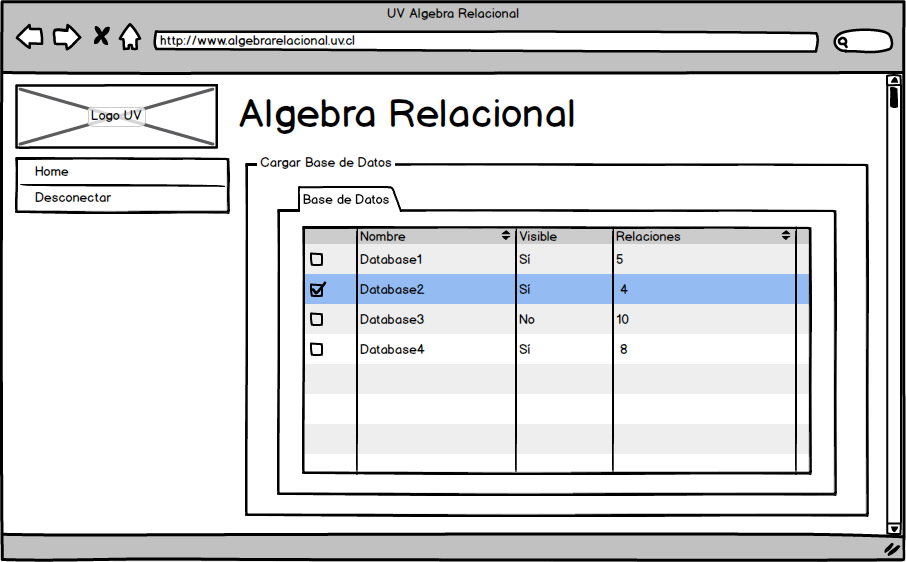
\includegraphics[width=13cm]{imagenes/cargar_bd.png}
\caption{Interfaz Cargar BD.}
\label{fig:cargarbd}
\end{figure}

\begin{figure}[h!]
\centering
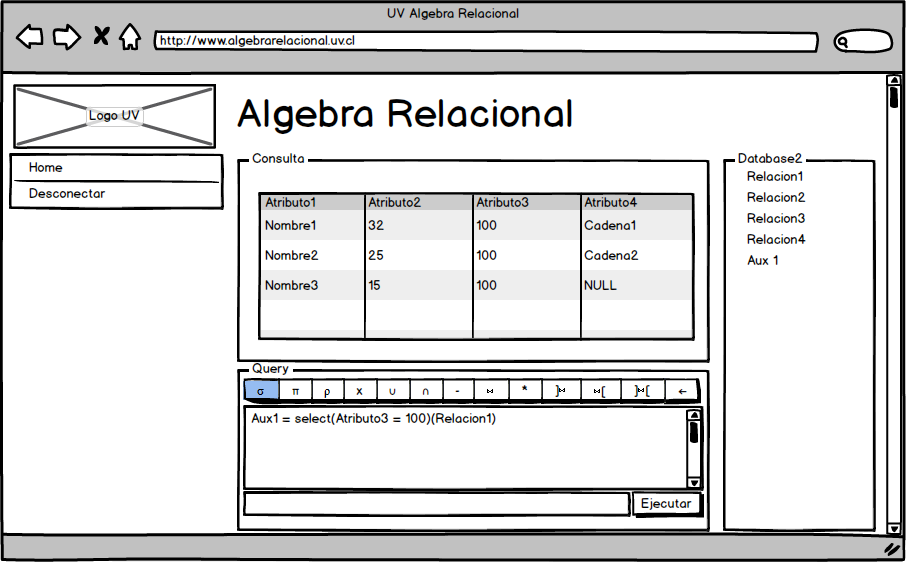
\includegraphics[width=13cm]{imagenes/hacer_consulta.png}
\caption{Interfaz Hacer Consulta.}
\label{fig:hacerconsulta}
\end{figure}

\clearpage
\begin{figure}[h!]
\centering
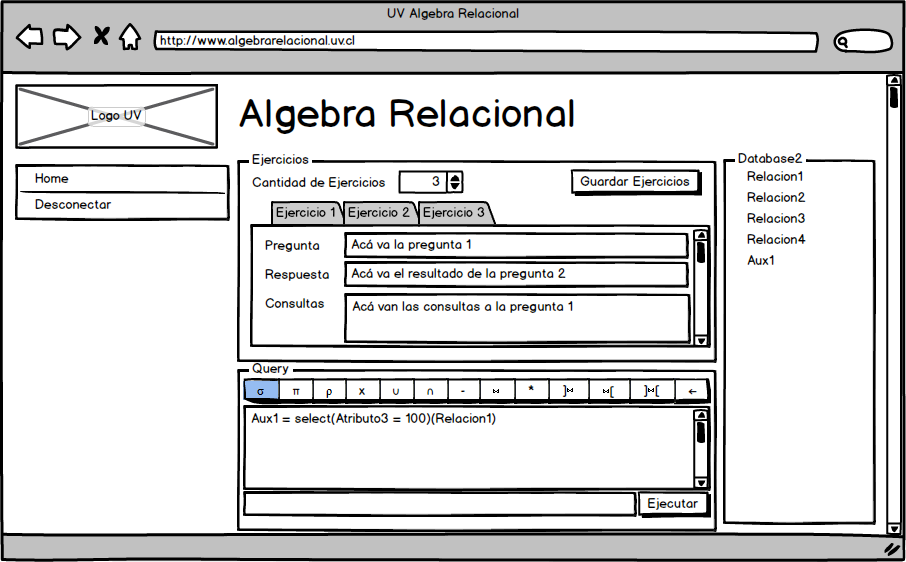
\includegraphics[width=13cm]{imagenes/crear_ejercicio.png}
\caption{Interfaz Crear Ejercicios.}
\label{fig:crearejercicios}
\end{figure}

\begin{figure}[h!]
\centering
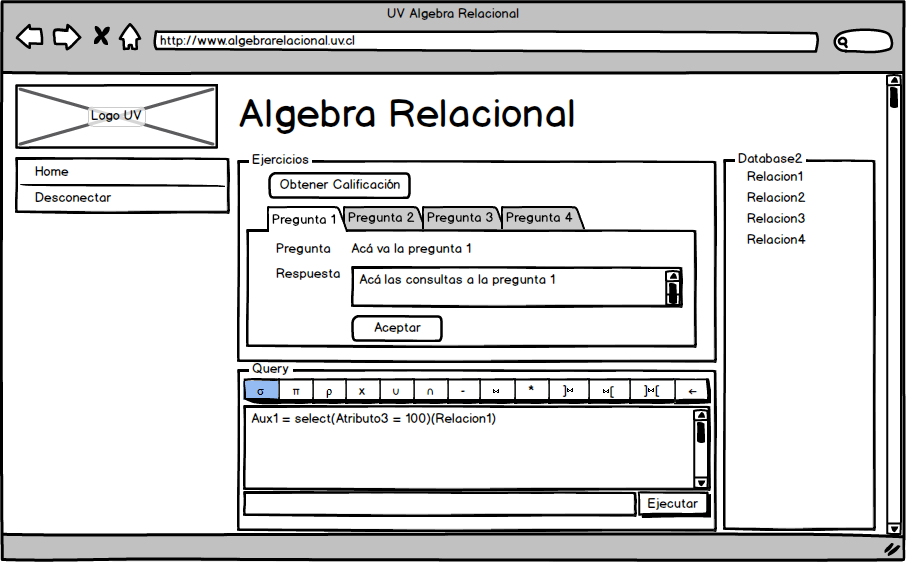
\includegraphics[width=13cm]{imagenes/responder_ejercicios.png}
\caption{Interfaz Responder Ejercicios.}
\label{fig:responderejercicios}
\end{figure}
